%!TeX root=../thesis.tex

\chapter{Implementasi dan Pengujian}

Pembahasan pada bab ini akan dibagi menjadi dua bagian. Bagian pertama dipaparkan tentang lingkungan dan detail implementasi. Sedangkan bagian kedua dibahas mengenai teknis dan hasil pengujian terhadap perangkat lunak yang sudah dibangun.

\section{Implementasi}

  Bagian implementasi dibagi menjadi tiga bagian. Bagian pertama dibahas mengenai lingkungan implementasi. Bagian kedua dibahas mengenai batasan implementasi. Bagian terakhir dibahas mengenai spesifikasi komponen.

  \subsection{Lingkungan Implementasi}

    Dalam proses implementasi digunakan sebuah komputer dan sejumlah perangkat lunak untuk menyelesaikan perangkat lunak yang dibangun. Detil spesifikasi perangkat keras dan lunak yang digunakan adalah seperti pada Tabel IV.1.
    
    \begin {table}[h]
\begin{center}
\caption {Spesifikasi Lingkungan Implementasi}
\begin{tabular}{|l|l|}

\hline
\rowcolor{gray!10}
Komponen & Spesifikasi \\
\hline

Sistem Operasi & Ubuntu 16.04.2 AMD 64-bit \\
\hline

CPU & Intel{\textregistered} Core{\texttrademark} i7-7500U CPU @ 2.70GHz × 4 \\
\hline

Host RAM & 16 GB \\
\hline

GPU & NVidia GeForce 940MX Compute Capablity 4.0 \\
\hline

Media Penyimpanan & \emph{Solid state drive} Samsung EVO 850 1TB \\
\hline

Dedicated Video RAM & 2 GB \\
\hline

CUDA Runtime & CUDA 8.0 r2 \\
\hline

G++ Compiler & GCC ??? \\
\hline

\end{tabular}
\end{center}
\end{table}


  \subsection{Batasan Implementasi}

    Implementasi dilakukan dengan batasan-batasan sebagai berikut.

    \begin{enumerate}

      \item Implementasi hanya mengerjakan komponen MPSE (\emph{multipattern search engine}) pada Snort

      \item Pencocokan menggunakan satu \emph{instance} GPU
    
      \item Pencocokan hanya dilakukan pada satu \emph{thread kernel code}
    
      \item Akuisisi \emph{payload} hanya dilakukan dari berkas PCAP

    \end{enumerate}

  \subsection{Spesifikasi Komponen}

    Berdasarkan analisis pada Bab III, implementasi akan berbasis implementasi \cite{lin2013} dengan skema \emph{pinned memory buffer} seperti pada \cite{gnort2008}. Implementasi dilakukan dengan membuat beberapa komponen, yaitu:

    \begin{enumerate}

      \item
      \emph{Handle} \\
      \emph{Handle} merupakan struktur data yang membungkus fungsionalitas pencocokan untuk dapat digunakan pada \emph{pipeline} Snort. \emph{Handle} berisi daftar pola, \emph{buffer} masukan, tabel transisi (sisi \emph{host} maupun \emph{device}), jumlah \emph{state} akhir dan \emph{list} hasil pencocokan. \emph{Buffer} masukan hanya dialokasi sekali sebesar 256 MB
      
      \emph{Handle} juga berisi fungsi-fungsi yang terkait modul yang dikembangkan seperti menambahkan pola, pembentukan kamus, pencocokan, dan mencetak informasi spesifik \emph{handle}. Fungsi-fungsi pada \emph{handle} akan memanggil modul lain yang terkait, misalnya fungsi pembentukan kamus akan memanggil komponen pembentukan kamus pada kode PFAC yang dibuat.      

      \item
      \emph{State machine builder} \\
      \emph{State machine builder} merupakan modul yang digunakan membentuk kamus untuk pencocokan. \emph{State machine} dibentuk di memori \emph{host}. Pola dikumpulkan dahulu dalam sebuah \emph{list}. Kemudian tiap pola akan dilakukan penelusuran DFS (\emph{depth-first search}) untuk membangun transisi tiap \emph{state}. 
      
      Dalam penelusuran, simpul baru akan terbentuk ketika simpul hasil transisi karakter tidak terdefinisi (bernilai \emph{null}). Untuk mengurangi \emph{lookup} ke \emph{global memory}, \emph{final state} tidak disebutkan secara eksplisit. Melainkan, dengan mengubah susunan nomor \emph{state} sehingga \emph{state} akhir berada pada nomor awal. Sehingga pengecekan hanya tinggal membandingkan nomor \emph{state} dengan jumlah \emph{state} akhir.

      \item
      \emph{Matcher wrapper} \\
      \emph{Matcher wrapper} adalah \emph{wrapper} dari \emph{kernel} sebelum dijalankan. \emph{Wrapper} akan menyiapkan \emph{payload} masukan sebelum \emph{kernel} dijalankan. Masukan disalin dari \emph{host buffer} ke \emph{device buffer}. Setelah persiapan selesai, \emph{wrapper} akan memanggil kode \emph{kernel} untuk menjalankan pencocokan. Setelah pencocokan selesai dilakukan, \emph{wrapper} akan menyalin \emph{array} hasil dari \emph{device} ke \emph{host}. \emph{Array} hasil tadi akan dikirim ke \emph{reducer} untuk digabungkan.
      
      \item
      \emph{Kernel code} \\
      \emph{Kernel} adalah kode GPU yang akan dijalankan untuk pencocokan. \emph{Kernel} hanya akan melakukan \emph{looping} terhadap nomor \emph{state} berdasarkan tabel transisi yang telah dimuat. \emph{Looping} akan berhenti ketika \emph{state} telah menuju \emph{state} akhir maupun status \emph{dummy}. Kemudian \emph{state} akhir akan ditulis ke \emph{output array}. \emph{Buffer} akan dibagi menjadi 4 bagian sebagai titik mulai pencocokan. Sehingga tiap \emph{thread} akan mencocokkan sebanyak 4 kali. \emph{Pseudocode} dari kode \emph{kernel} akan terlihat seperti pada Gambar IV.1 berikut.

      \begin{figure}[htb]
        \centering
        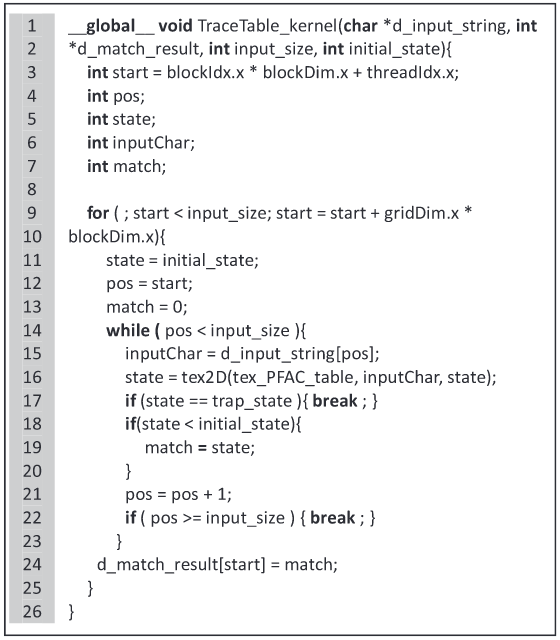
\includegraphics[width=0.65\textwidth]{resources/pseudo.png}
        \caption[\emph{Pseudocoode kernel}]{\emph{Pseudocoode kernel}}
      \end{figure}

      \item
      \emph{Reducer} \\
      \emph{Reducer} akan menggabungkan hasil pencocokan dari tiap \emph{thread} sehingga diperoleh total kumpulan pola yang terdeteksi. \emph{Reducer} dipanggil setelah \emph{matcher} dijalankan. \emph{Reducing} akan dilakukan secara sekuensial pada CPU. Hasil \emph{reducing} akan dikembalikan ke fungsi \emph{search} milik \emph{handle} untuk dikembalikan lagi ke Snort dalam bentuk jumlah.
      
    \end{enumerate}

  % \subsection{Konfigurasi}

  %   Agar Snort dapat dijalankan dengan modul yang telah diintegrasikan, perlu dibuat pengubahan pada konfigurasi. Konfigurasi akan disuplai dari skrip lua. Diantara poin yang perlu diubah pada berkas konfigurasi yaitu:

  %   \begin{enumerate}
  %     \item Pencocokan dilakukan dengan modul PFAC yang telah selesai diintegrasikan.
  %     \item Modul \emph{daq (data acquisition)} yang digunakan hanya pcap-daq untuk dapat membaca berkas PCAP.
  %     \item \emph{Ruleset} diatur menunjuk ke lokasi \emph{rule} Talos.
  %     \item \emph{Buffer} untuk \emph{payload} diatur sebesar 128 kB.
  %   \end{enumerate}

\section{Pengujian}

  \subsection{Tujuan Pengujian}
    Pengujian dilakukan untuk mendapatkan perbandingan kinerja antara modul yang dikembangkan dan modul yang ada dalam NIDS Snort. Pengujian dibatasi dengan menggunakan konfigurasi \emph{data acquisition} PCAP dengan masukan \emph{file} tcpdump saja. \emph{Live testing} tidak diujikan dalam Tugas Akhir ini mengingat kapasitas \emph{network interface} dapat menjadi \emph{bottleneck} sehingga hasil perbandingan tidak akurat.

  \subsection{Skenario Pengujian}
  
    Pengujian dilakukan untuk mengukur peningkatan kinerja deteksi Snort. Skenario yang akan diujikan meliputi strategi-strategi yang dibahas pada Subbab III.2. Berikut ini adalah tipe-tipe skenario yang diuji dalam pengujian ini.

    \begin{enumerate}
      
      \item \emph{Baseline} (Aho-Corasick dengan \emph{multithreading} CPU) \\
      \emph{Baseline} akan menggunakan konfigurasi default Snort. Ini menjadi dasar pengukuran kinerja dan kebenaran program yang diimplementasikan pada GPU.

      \item Skenario 1 (PFAC dengan \emph{global memory}) \\
      Skenario ini adalah skenario paling dasar. Optimasi hanya dilakukan pada algoritma tanpa melibatkan optimasi pada latensi GPU.

      \item Skenario 2 (PFAC dengan \emph{shared memory}) \\
      Skenario ini memanfaatkan \emph{shared memory} untuk mengurangi akses ke \emph{global memory}. Transisi \emph{state} awal ke tiap huruf serta \emph{stream} masukan ditampung dalam \emph{shared memory}.

      \item Skenario 3 (PFAC dengan \emph{shared memory} dan \emph{pinned memory}) \\
      Skenario ini mirip dengan skenario 2 dengan tambahan \emph{pinned memory} pada \emph{buffer}. Mekanisme ini diharapkan dapat mengurangi \emph{swappiness} dan memungkinkan DMA (\emph{direct memory access}).

      \item Skenario 4 (PFAC dengan \emph{shared memory}, \emph{pinned memory}, dan \emph{texture memory}) \\
      Skenario ini mirip dengan skenario 3 dengan tambahan \emph{texture memory} pada kamus. Dengan \emph{cache} yang lebih besar, penggunaan \emph{texture memory} diharapkan mengurangi transfer memori.

    \end{enumerate}

    Kelima skenario akan diuji dengan ukuran \emph{buffer} berbeda, yaitu 128 kB (bawaan), 512 kB, 1024 kB, dan 2018 kB.

  \subsection{Lingkungan Pengujian}

    Pengujian dilakukan pada komputer dengan spesifikasi seperti pada Tabel IV.2 berikut.
    
    \begin {table}[h]
\begin{center}
\caption {Spesifikasi Lingkungan Pengujian}
    \begin{tabular}{|l|l|}

\hline
\rowcolor{gray!15}
Komponen & Spesifikasi \\
\hline

Sistem Operasi & Ubuntu 16.04.5 amd64 \\
\hline

CPU & Intel Core i7-7500U CPU @ 2.70GHz × 4 \\
\hline

\emph{Host} RAM & 16 GB \\
\hline

Media Penyimpanan & SSD SATA III 6 Gbps \\
\hline

GPU & NVIDIA GeForce 940MX \\
\hline

Arsitektur GPU & Maxwell \\
\hline

\emph{Compute Capability} & 5.0 \\
\hline

\emph{Dedicated Video} RAM & 2 GB \\
\hline

CUDA \emph{Runtime} & CUDA 8.0 r2 \\
\hline

C/C++ \emph{Compiler} & GCC 5.4.0 \\
\hline

\end{tabular}

\end{center}
\end{table}


  \subsection{Hasil Pengujian}

    Berikut merupakan hasil pengujian dari seluruh skenario di atas. \emph{Ruleset} yang digunakan yaitu Snort VRT \emph{ruleset} versi 3000. Sedangkan berkas masukan didapatkan dari \emph{log traffic} kompetisi DEFCON 25 yang berlangsung pada bulan Juli tahun 2017. Dataset didapatkan dari jaringan \emph{torrent} milik arsip DEFCON berupa beberapa berkas PCAP sebesar sekitar 2,6 GB. Berikut adalah hasil pengujian pada ukuran \emph{buffer} berbeda.\clearpage

    \begin {table}[h]
\begin{center}
\caption {Hasil Pengujian}

    \begin{tabular}{|p{4cm}|p{4cm}|p{4cm}|}

    \hline
    \rowcolor{gray!10}
    Skenario & Runtime (detik) & Speedup \\
    \hline

    \emph{Baseline} & 94.631856 & 1 \\
    \hline
    
    Skenario 1 & 424.277725 & 0.21 \\
    \hline
    
    Skenario 2 & 265.578648 & 0.4 \\
    \hline
    
    Skenario 3 & 265.913109 & 0.4 \\
    \hline

    \end{tabular}

\end{center}
\end{table}
  

  \subsection{Analisis Hasil Pengujian}
    
    Dari hasil pengujian, didapatkan bahwa hasil skenario 1 memilki kapasitas paling rendah. Alasannya yaitu karena operasi pencocokan \emph{string} adalah operasi yang \emph{memory-bound}. Diperlukan banyak akses ke penyimpanan kamus untuk mendapatkan transisi ke \emph{next state}. Karena kamus disimpan di \emph{global memory}, maka \emph{fetch} ke \emph{global memory} menjadi sering dan menimbulkan latensi yang cukup besar.
    
    Skenario 2 secara umum lebih cepat beberapa kali daripada skenario 1, yaitu sekitar 15 kali lipat lebih cepat. Hal ini karena kecepatan akses \emph{global memory} lebih besar dari \emph{shared memory}. Dalam skenario ini, \emph{input string} seharusnya tidak berpengaruh banyak karena adanya \emph{coalescing access}. Sehingga pemuatan baris transisi dari \emph{state} awal ke \emph{shared memory} memiliki pengaruh yang besar terhadap \emph{throughput} sistem. Ini menunjukkan bahwa mayoritas \emph{thread} akan berhenti pada awal pencocokan.

    Skenario 3 tidak terlalu berpengaruh terhadap skenario 2. Keuntungan \emph{pinned memory} tidak terlalu terlihat bahkan cenderung memperlambat. Sejalan dengan eksperimen yang dilakukan \cite{gnort2008}. Ini karena \emph{pinned memory} memiliki \emph{overhead} saat alokasi dan dealokasi. Kemungkinan besar ini terjadi karena ukuran \emph{buffer} belum terlalu besar. \emph{Overhead} saat alokasi masih belum sebanding dengan perbedaan \emph{transfer} antara DMA dan melalui CPU. Selain itu, juga tidak terjadi \emph{swap} terhadap \emph{page} yang terdapat \emph{buffer} karena ukuran memori masih kecil.

    Sedangkan skenario 4 baru terlihat perbedaan signifikan terhadap skenario 2 dan 3 pada \emph{buffer} sebesar 1 MB ke atas. Terlihat bahwa adanya \emph{cache} pada memori tekstur membantu menurunkan akses ke memori global dan meningkatkan kinerja keseluruhan modul. 